\section{Algoritmos y aplicaciones}

El problema es de visión por computadora: la entrada es una imagen de $224\times224\times3=150{,}528$ valores y la salida es una de 104 clases. En esta sección explicamos por qué las redes convolucionales son la familia adecuada, proponemos dos arquitecturas concretas, explicamos qué papel pueden tener los métodos tradicionales y describimos las aplicaciones posibles.

\subsection{Por qué redes neuronales convolucionales}

Las redes neuronales convolucionales (CNN) aplican filtros pequeños (por ejemplo, de $3\times3$) que recorren toda la imagen. En las primeras capas estos filtros aprenden a detectar bordes y cambios de color; en las capas profundas, combinaciones de ellos, como texturas, pétalos o discos centrales (Figura~\ref{fig:cnn_diagram}). En las capas internas se usa la activación ReLU y en la salida Softmax, que convierte los 104 valores finales en probabilidades.

\begin{figure}[H]
    \centering
    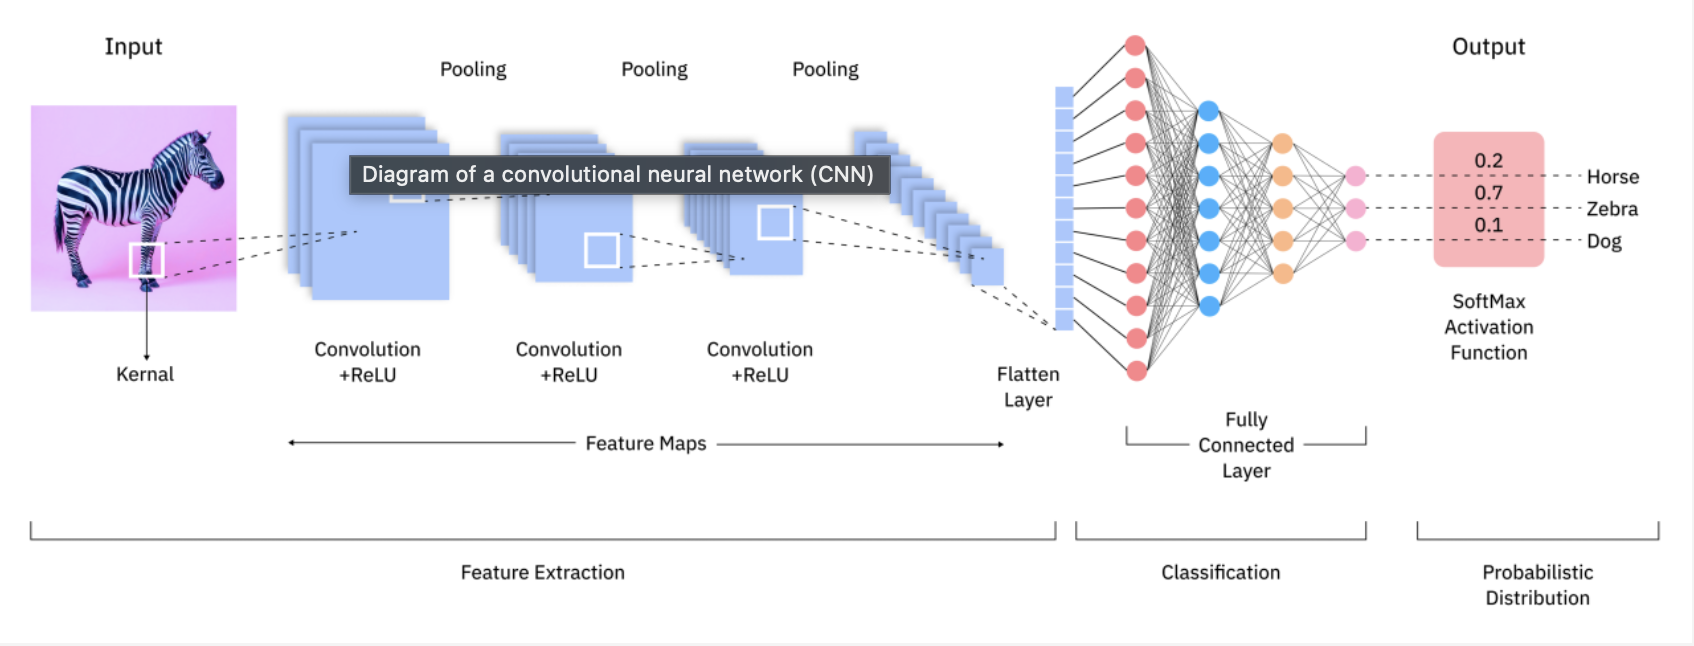
\includegraphics[width=0.9\textwidth]{cnn_diagram.png}
    \caption{Una CNN descompone la imagen en mapas de características y después las combina para clasificar \parencite{ibmWhatImage}.}
    \label{fig:cnn_diagram}
\end{figure}

Para este conjunto de datos, la CNN tiene dos ventajas concretas sobre una red densa:
\begin{itemize}
    \item \textbf{Comparte parámetros.} Una capa convolucional de 32 filtros de $3\times3$ sobre una imagen RGB tiene $3\cdot3\cdot3\cdot32+32=896$ parámetros, sin importar el tamaño de la imagen. Una capa densa de 256 neuronas conectada directamente a los 150,528 valores tendría $150{,}528\cdot256+256\approx38.5$ millones, más de 3,000 parámetros por cada imagen de entrenamiento.
    \item \textbf{Reconoce un patrón en cualquier posición.} El mismo filtro se aplica en toda la imagen, así que una flor se reconoce aunque aparezca en una esquina o en el centro, algo indispensable porque nuestras fotos cambian mucho de escala y encuadre.
\end{itemize}

La desventaja es el costo de cómputo, ya que entrenar una CNN requiere muchas operaciones por imagen. Por eso la competencia ofrece TPU y por eso también buscamos arquitecturas eficientes.

\subsection{Propuesta 1: CNN propia como línea base}

La primera arquitectura es una CNN diseñada por nosotros y entrenada desde cero. Su objetivo es medir cuánto se puede aprender usando únicamente las 12,753 imágenes de entrenamiento y servir de referencia para la segunda propuesta. La arquitectura es:

\begin{enumerate}
    \item Cuatro bloques convolucionales con 32, 64, 128 y 256 filtros. Cada bloque tiene una convolución de $3\times3$, normalización por lotes (\textit{batch normalization}), ReLU y \textit{max pooling} de $2\times2$, que reduce a la mitad el alto y el ancho. Así la red pasa de $224\times224$ a mapas de $14\times14$ con 256 canales.
    \item \textit{Global Average Pooling}, que resume cada uno de los 256 mapas en un solo número.
    \item Una capa densa de 256 neuronas con ReLU y \textit{Dropout} de 0.5 para reducir el sobreajuste.
    \item Una capa de salida de 104 neuronas con Softmax.
\end{enumerate}

En total son aproximadamente 0.48 millones de parámetros, una cantidad pequeña a propósito. Con una mediana de 88 imágenes por clase y 24 clases con menos de 30, una red grande entrenada desde cero memorizaría el conjunto de entrenamiento. Para compensar la falta de datos usaremos aumento de datos (volteos, rotaciones pequeñas, recortes y cambios de brillo) solo en entrenamiento.

Esperamos que esta red aprenda bien las clases grandes y fáciles (como \textit{sunflower}), pero que tenga problemas con las clases pequeñas y con las que se parecen entre sí (Tabla~\ref{tab:ejemplos}), porque necesita aprender desde cero incluso los bordes y texturas más básicos.

\subsection{Propuesta 2: aprendizaje por transferencia con EfficientNetB0 o ResNet50}

La segunda arquitectura reutiliza una red ya entrenada en ImageNet, un conjunto de 1.28 millones de imágenes de 1,000 categorías \parencite{russakovsky2015}. Esta es la propuesta principal, por tres razones:

\begin{itemize}
    \item \textbf{Las primeras capas sirven para cualquier imagen.} Los filtros iniciales de una red entrenada en ImageNet detectan bordes, colores y texturas que son útiles en otras tareas, y transferirlos mejora el resultado aun cuando la tarea nueva es distinta \parencite{yosinski2014}. Con aproximadamente 123 imágenes por clase no podríamos aprender esos filtros nosotros mismos; al heredarlos, solo hay que aprender a combinarlos para distinguir 104 flores.
    \item \textbf{Ya se probó con flores.} En Oxford 102, de donde vienen 102 de nuestras 104 clases, usar las características de una CNN entrenada en ImageNet con un clasificador lineal alcanzó 86.8\,\% de exactitud promedio \parencite{razavian2014}, frente a 72.8\,\% del método original con características diseñadas a mano \parencite{nilsback2008}.
    \item \textbf{Pocos parámetros nuevos.} Se retira la capa de salida de ImageNet y se agrega una nueva de 104 clases. Sobre las 1,280 características de EfficientNetB0, esta capa tiene $1{,}280\cdot104+104=133{,}224$ parámetros, que sí se pueden ajustar bien con 12,753 imágenes.
\end{itemize}

Elegimos \textbf{EfficientNetB0} como primera opción y \textbf{ResNet50} como alternativa (Tabla~\ref{tab:preentrenadas}). EfficientNetB0 escala de forma equilibrada la profundidad, el ancho y la resolución de la red, y por eso obtiene mayor exactitud en ImageNet con 5 veces menos parámetros que ResNet50 \parencite{tan2019}. ResNet50 introduce conexiones residuales, que suman la entrada de cada bloque a su salida y permiten entrenar redes profundas sin que el gradiente se desvanezca \parencite{he2016}; es más pesada, pero es una arquitectura muy estudiada y sirve para confirmar que los resultados no dependen de una sola red. Ambas usan entradas de $224\times224$, que es una de las resoluciones que trae el conjunto de datos.

\begin{table}[H]
\centering
\caption{Redes preentrenadas consideradas \parencite{tan2019}.}
\label{tab:preentrenadas}
\begin{tabular}{lrrrr}
\toprule
Red & Parámetros & Entrada & Exactitud top-1 & Características \\
 & (millones) & (píxeles) & ImageNet (\%) & tras el \textit{pooling} \\
\midrule
EfficientNetB0 & 5.3 & $224\times224$ & 77.1 & 1,280 \\
ResNet50 & 26 & $224\times224$ & 76.0 & 2,048 \\
\bottomrule
\end{tabular}
\end{table}

El entrenamiento se hará en dos fases:
\begin{enumerate}
    \item \textbf{Extracción de características.} Se congelan los pesos de la red preentrenada y solo se entrena la nueva capa de salida (con \textit{Dropout} antes de ella). Así se evita que los gradientes grandes del inicio dañen los filtros aprendidos en ImageNet.
    \item \textbf{Ajuste fino} (\textit{fine-tuning}). Se descongelan los últimos bloques y se entrena toda la parte superior con una tasa de aprendizaje baja (del orden de $10^{-5}$), para adaptar las características de alto nivel a las flores sin olvidar las de bajo nivel.
\end{enumerate}

En ambas fases se usará el mismo aumento de datos que en la propuesta 1 y el preprocesamiento que pide cada red. Además, para atender el desbalance, compararemos la entropía cruzada normal contra una ponderada por clase, y elegiremos el modelo por su F1 macro en validación.

\subsection{Métodos tradicionales: solo sobre características}

Los métodos clásicos de aprendizaje automático no son adecuados si se aplican directamente sobre los píxeles, porque cada imagen sería un vector de 150,528 dimensiones y solo tenemos 12,753 ejemplos, es decir, más dimensiones que ejemplos:

\begin{description}
    \item[k vecinos más cercanos (KNN)] Clasifica una imagen según la clase de las $k$ imágenes más cercanas, normalmente con distancia euclidiana. Sobre píxeles, esa distancia mide si dos fotos tienen colores parecidos en las mismas posiciones, no si muestran la misma flor: dos fotos de girasoles con distinto encuadre quedan lejos, y un girasol y una rudbeckia sobre fondo verde quedan cerca. Además, en dimensiones tan altas las distancias entre todos los puntos tienden a parecerse.
    \item[Bosque aleatorio] Combina muchos árboles de decisión, cada uno entrenado con una muestra distinta de los datos, y clasifica por votación. Cada división del árbol pregunta por el valor de un píxel en una posición fija, pero la flor no aparece siempre en la misma posición, así que esas reglas no generalizan.
    \item[Máquinas de vectores de soporte (SVM)] Buscan el hiperplano que separa dos clases con el mayor margen; para 104 clases se entrena un clasificador por clase (uno contra todos). Sobre píxeles, un SVM lineal tendría $104\cdot150{,}529\approx15.7$ millones de pesos, y seguiría sin ser robusto a cambios de posición o iluminación.
\end{description}

Estos métodos sí son útiles cuando reciben un vector de características compacto en lugar de los píxeles. Así trabajó el método original de Oxford 102, que usó un SVM sobre descriptores de color, forma (SIFT) y gradientes (HOG) \parencite{nilsback2008}. Del mismo modo, Razavian et al.\ obtuvieron su resultado de 86.8\,\% con un SVM lineal sobre las características de una CNN preentrenada \parencite{razavian2014}. Por eso los usaremos como comparación sobre los vectores de 1,280 características que produce EfficientNetB0: si un KNN o un SVM sobre esas características se acerca a la red con ajuste fino, sabremos cuánto aporta realmente el ajuste fino.

\subsection{Otras arquitecturas consideradas}

AlexNet fue la primera CNN profunda en ganar ImageNet, en 2012 \parencite{krizhevsky2012}, e Inception (GoogLeNet) introdujo bloques que aplican filtros de varios tamaños en paralelo \parencite{szegedy2015}. Ambas son importantes históricamente, pero no las elegimos: AlexNet tiene unos 60 millones de parámetros y menor exactitud que las redes de la Tabla~\ref{tab:preentrenadas}, y las versiones de Inception que superan a EfficientNetB0 requieren más parámetros y una entrada de $299\times299$. Si EfficientNetB0 resultara insuficiente, el siguiente paso sería una EfficientNet más grande con las imágenes de $331\times331$ o $512\times512$.

\subsection{Aplicaciones posibles}

Un modelo que clasifica flores a partir de imágenes responde directamente a las necesidades descritas en el contexto. La primera es la \textbf{identificación automática de plantas} en plataformas de ciencia ciudadana: iNaturalist, con más de 300 millones de observaciones, usa un modelo de visión por computadora entrenado con esas mismas observaciones para sugerir la especie a partir de una fotografía \parencite{inaturalist}. Sin ese apoyo, cada observación dependería de que una persona la revisara, y el monitoreo de biodiversidad sería lento y difícil de escalar. Este proyecto es una versión a menor escala de ese tipo de sistemas.

La segunda es una \textbf{herramienta educativa} para estudiantes o visitantes de jardines botánicos, que permita fotografiar una flor y consultar información sobre ella. La tercera es el \textbf{apoyo al comercio de flores}, por ejemplo para clasificar o verificar variedades comerciales como el clavel, que forma parte de las 104 clases.

Sin embargo, el modelo desarrollado solo podrá reconocer las 104 clases presentes en el conjunto de datos, por lo que una aplicación real más amplia requeriría entrenarlo con una mayor variedad de especies y con fotografías tomadas en las condiciones de uso reales.
